\chapter{Building a Model of the System}\label{chap:model}
With a theory of superconducting qubit readout and a set of parameters that describe our system with respect to this theory, we will in this chapter built up the simulation. We will will present this simulation work in three steps. First, we will take a look at four different methods of simulating the system. Next, we will argument for the use of the dispersive model compared to the full time-dependent Hamilton. Finally, we will adjust some parameters of the simulation such as the dimensions of our Hilbert Space and the size of the time steps.

\section{Different Simulation Approaches}
Throughout the first few chapter, we covered different ways of representing and numerically integrating a quantum system. In this chapter, we will summarize the few methods. Some of the properties are summed up in table \ref{tab:simulation_types}

\begin{itemize}
    \item \textbf{Unitary} - This is a time evolution of the Schrödinger Equation \ref{sec:scroedinger}. In Qutip this is done by the Adams algorithm which we covered in section \ref{sec:numerical_implementations}. This is the fastest and simplest to run, but does not support interaction with the environment.  
    \item \textbf{Lindblad Equation} - The Lindblad equation simulates the density matrix and allows us to include dissipation terms. Like the Schrödinger equation, the Lindblad Master Equation is also deterministic, so it is only necessary to run it once for each configuration. All dynamics can then be extracted from $\rho$. 
    \item \textbf{Monte Carlo} - The Monte Carlo method is described in sec \ref{sec:monte_carlo} and the main idea is that dissipation are applied stochastically and in between the dynamics are governed by the Schrödinger Equation. This allows for faster simulation than the Lindblad Master Equation. However, multiple trajectories will have to be taken to make sure the dynamics represent the full dynamics.
    \item \textbf{Stochastic Master Equation} - The Stochastic Master Equation is described in chapter \ref{chap:measurements} and the most complicated of the simulation tools. This includes the dynamics of the Lindblad Equation, but in addition also supports the weak measurement which is obtained during a readout.
\end{itemize}\todo{Citations}

\begin{margintable}[-10 cm]
    \centering
    \caption{Overview of what the different simulation schemes support. The abbreviations correspond to SE: Schödingers Equation, ME: Master Equation, MC: Monte Carlo, SME: Stochastic Master Equation}
    \vspace{0.3 cm}
    \begin{tabular}{c|c|c|c|c}
                    &  SE   & ME    & MC    & SME    \\ \hline 
    deterministic   & x     & x     &       &        \\
    dissipation     &       & x     & x     & x      \\ 
    mixed states    &       & x     &       & x      \\ 
    measurements    &       &       &       & x      \\ 
    state           & $\psi$& $\rho$&$\psi$ & $\rho$ \\
    state size      & $n$   & $n^2$ & $n$   & $n^2$
    \end{tabular}
    \label{tab:simulation_types}
\end{margintable}

\subsection{Comparing Simulations for $T_1$ Calibration}
\begin{figure*}[t]
    % \begin{minipage}{0.45\textwidth}
    \centering
    % 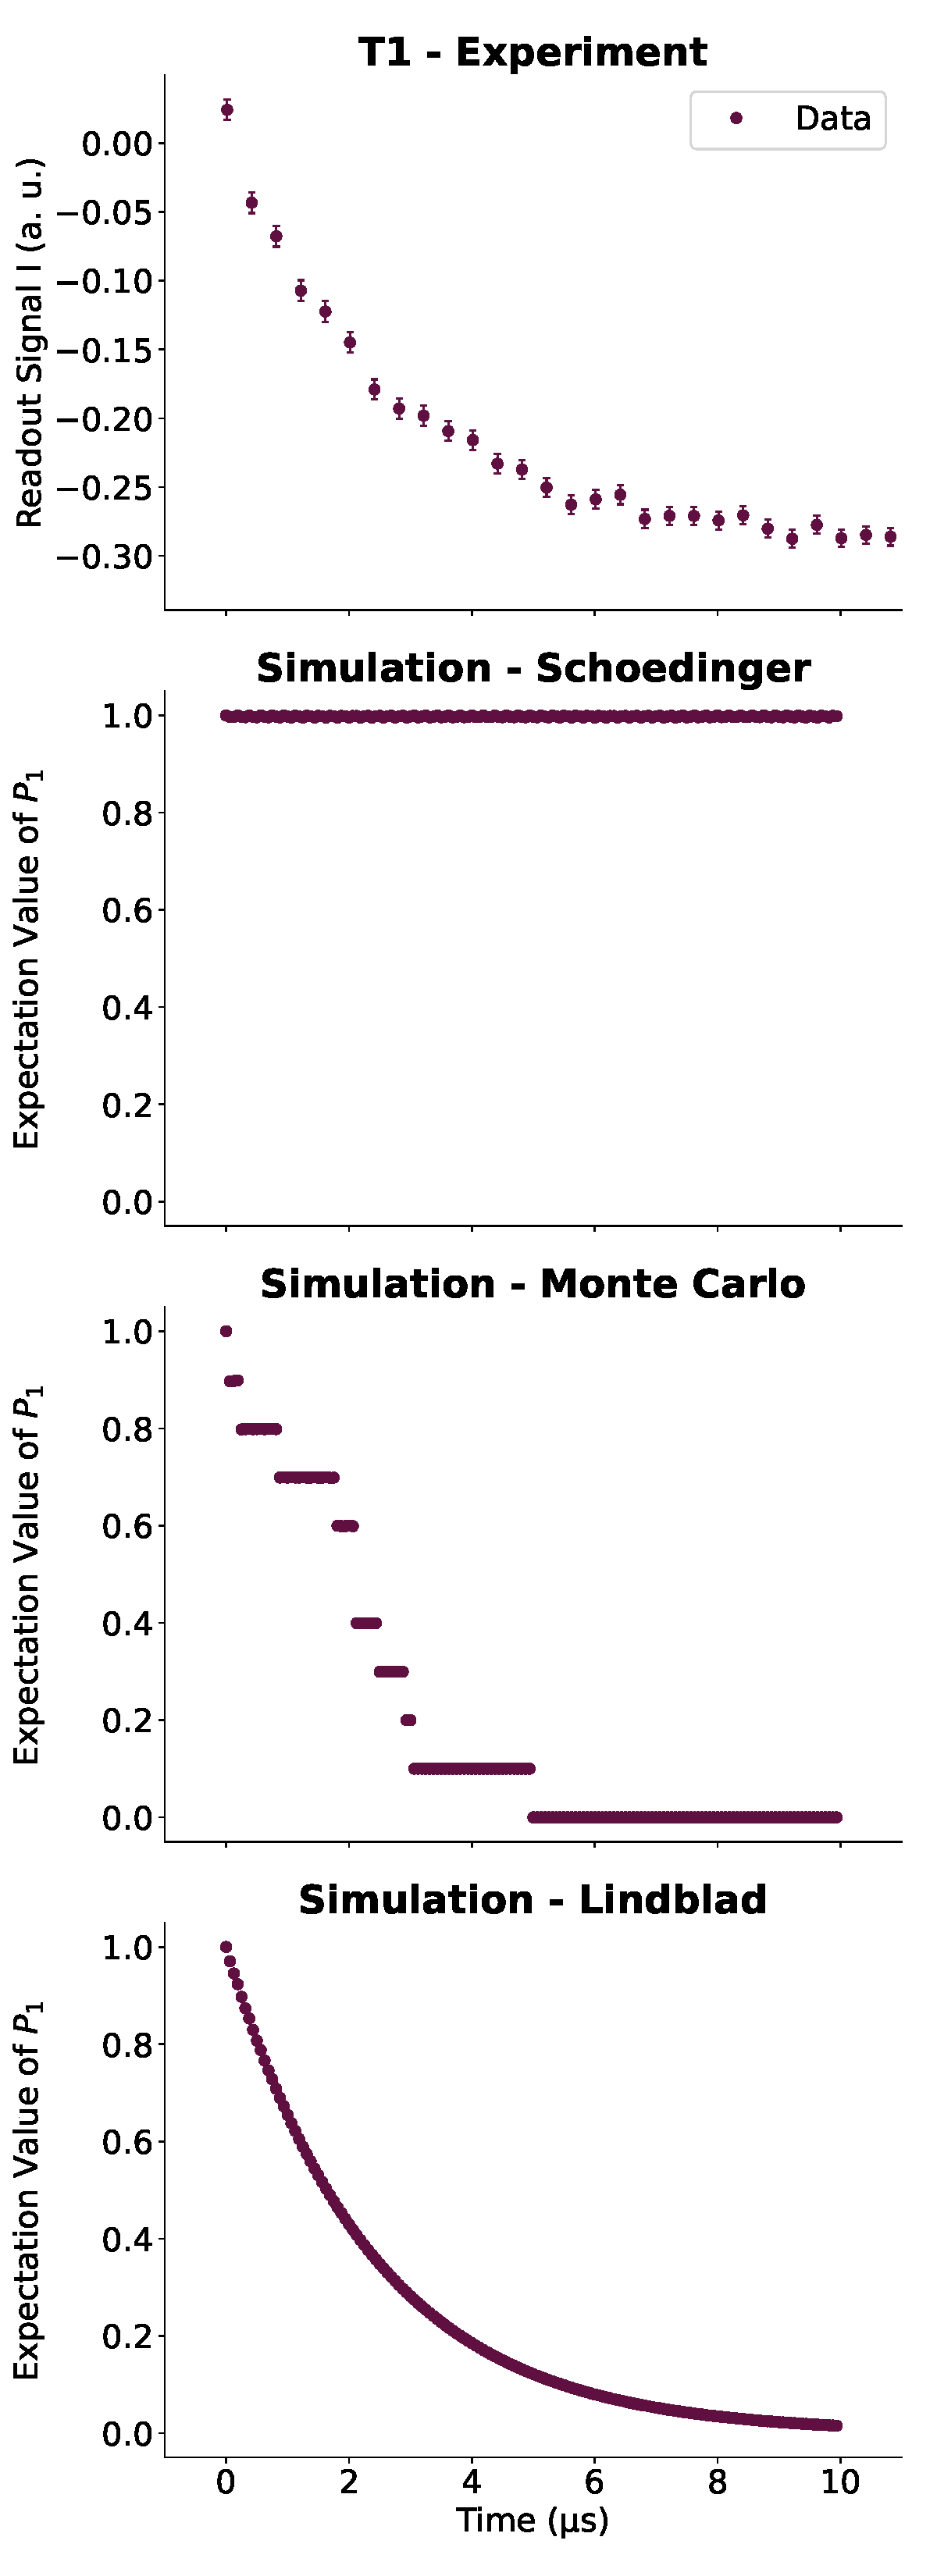
\includegraphics[]{Simulations/simulations_of_calibrations/Figs/qubit_T1.pdf}
    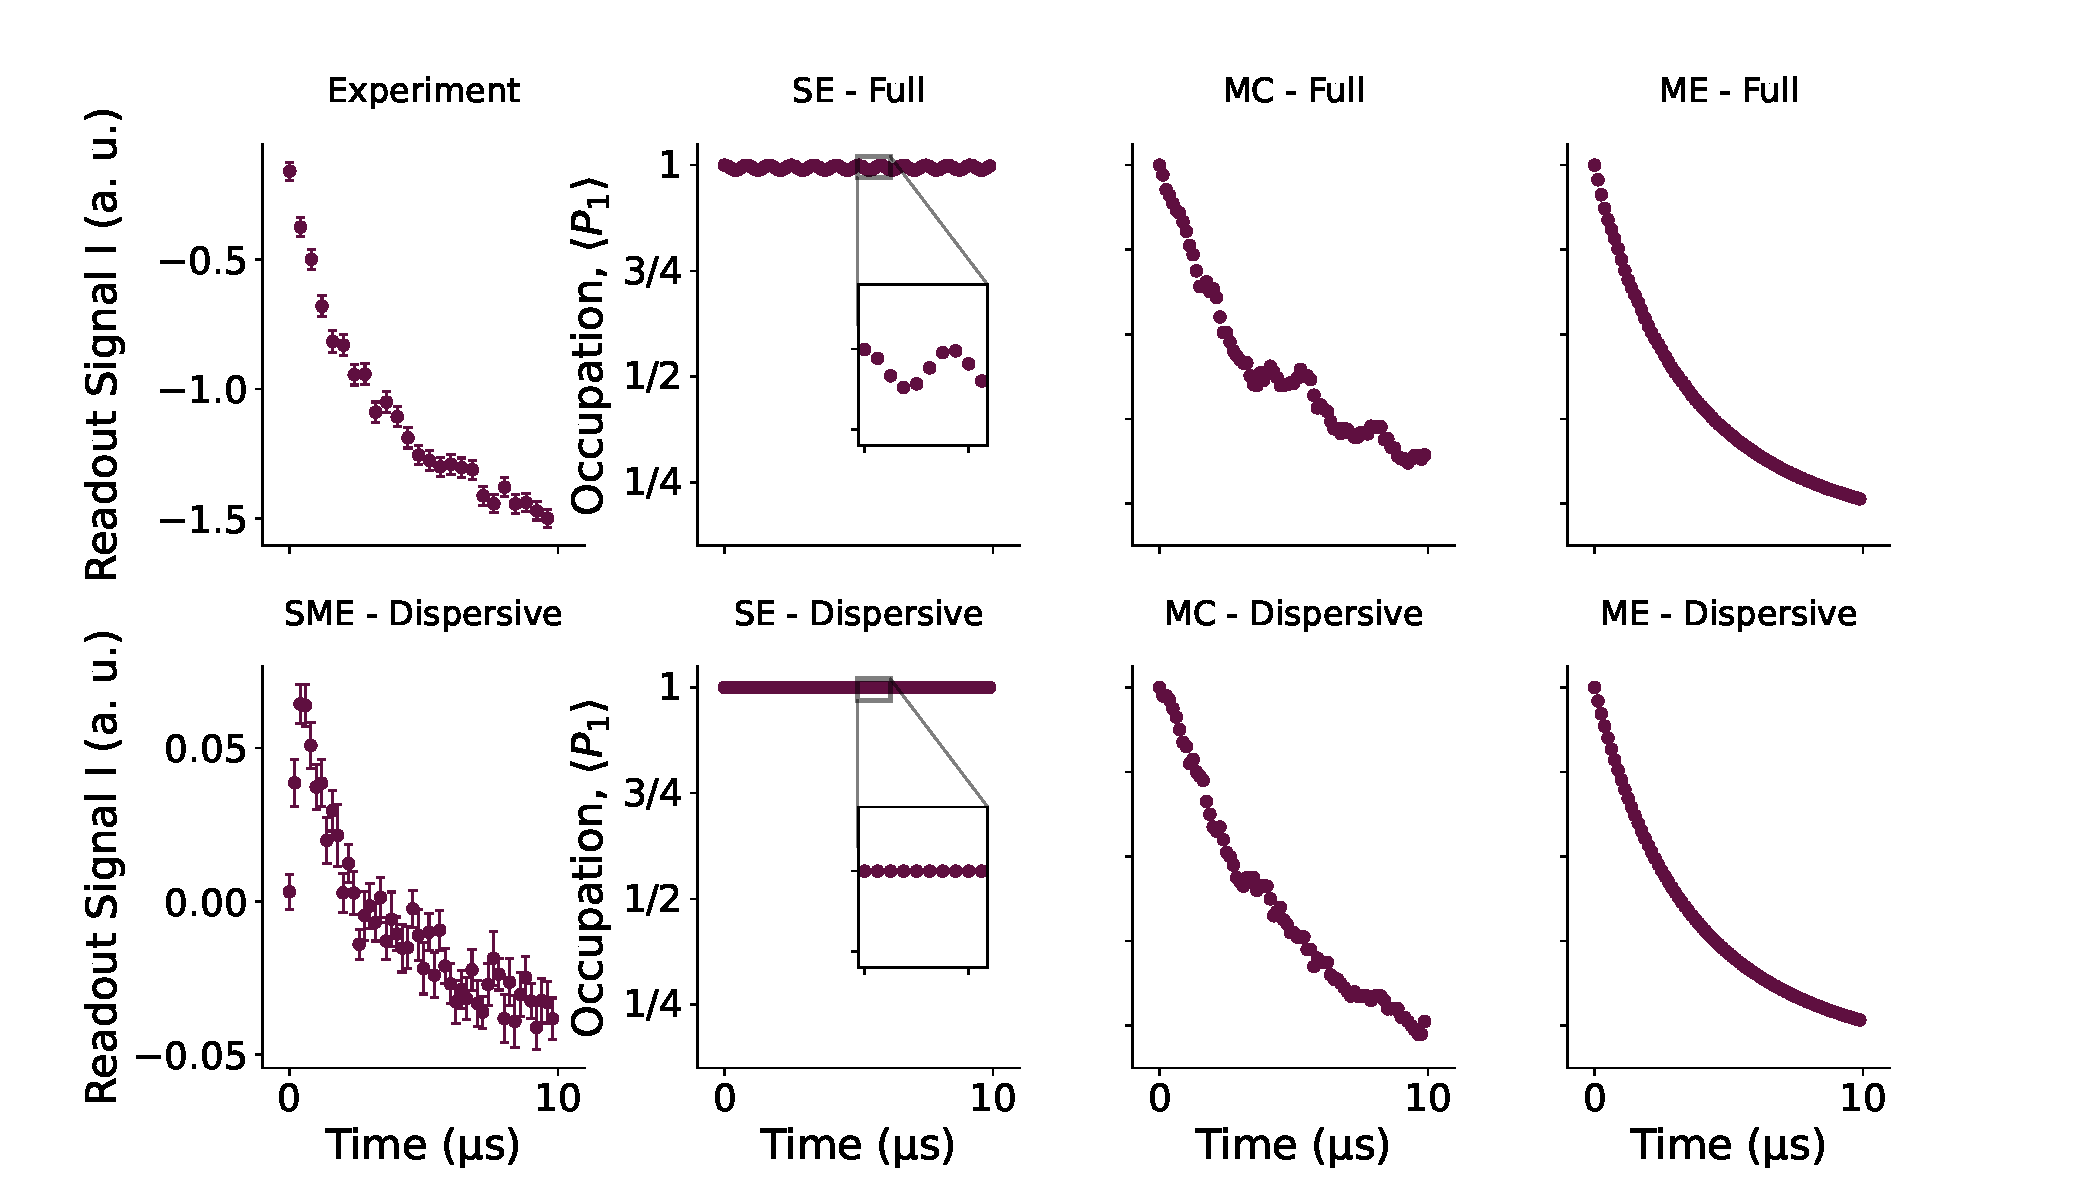
\includegraphics[]{Simulations/simulations_of_calibrations/Figs/qubit_T1_dispersive.pdf}
    % \end{minipage}
    %     \begin{minipage}{0.45\textwidth}
    %     \centering
    %     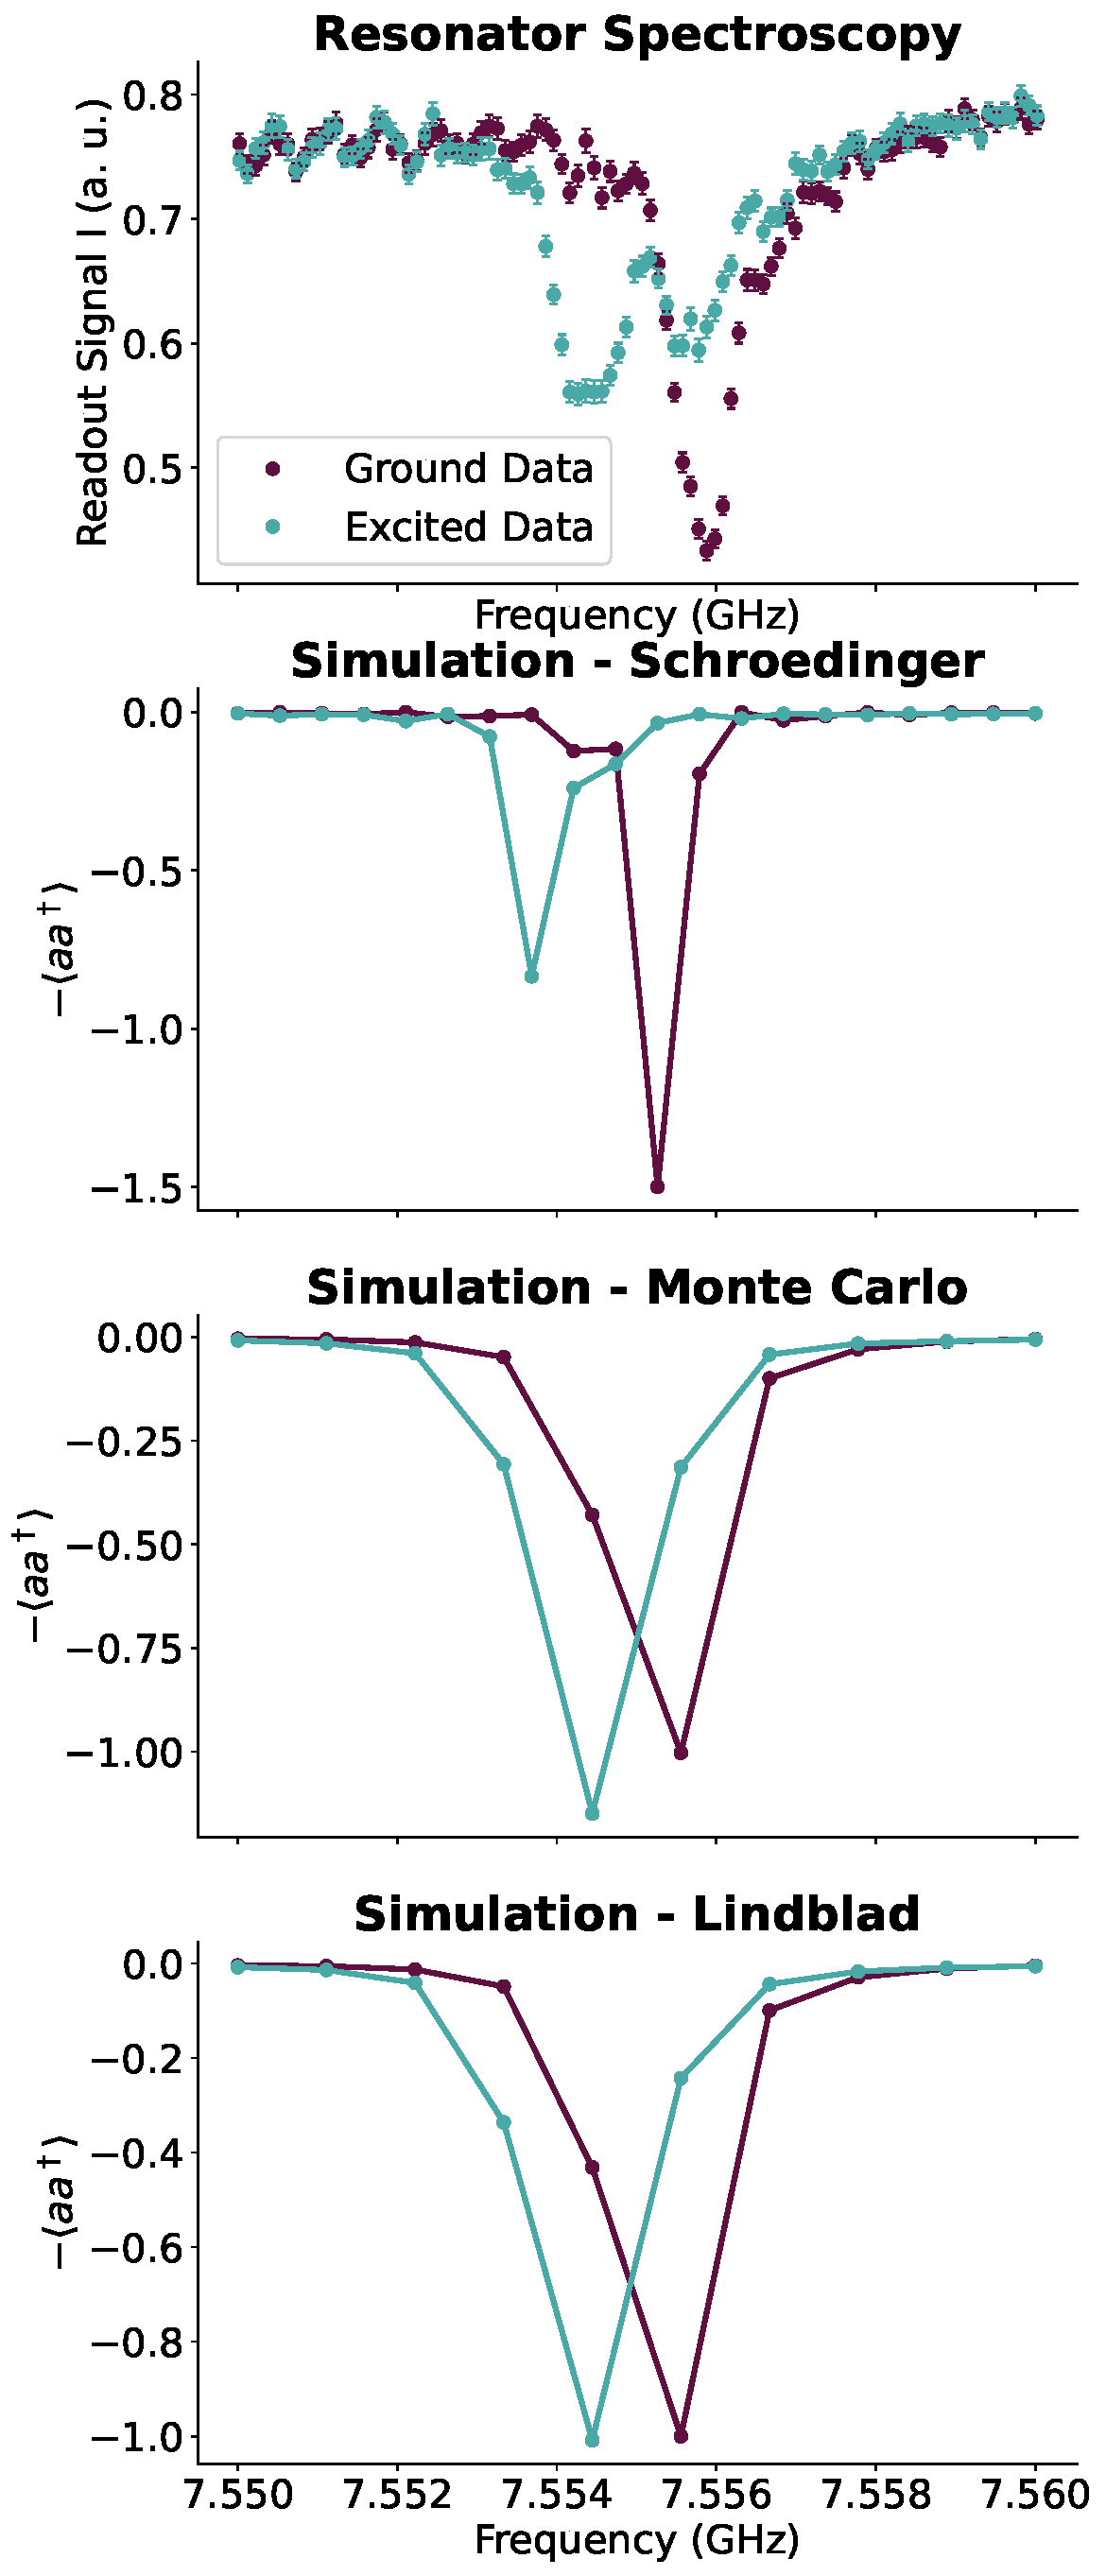
\includegraphics[]{Simulations/simulations_of_calibrations/Figs/resonator_spectroscopy.pdf}
    % \end{minipage}
    \caption{Illustration of the $T_1$ experiment run with different simulation techniques. In the Schrödinger experiment, a zoom-in is made to show the oscillations from qubit-resonator interaction which are not present in the dispersive model. }
    \label{fig:calibrations_in_simulation}
\end{figure*}
\begin{margintable}[2 cm]
    \caption{Running time of the different simulation approaches to running the $T_1$ calibration scheme.}
    \vspace{0.3 cm}
    \centering
    \begin{tabular}{r|llll}
                    &  SE   & ME    & MC    & SME   \\ \hline 
    Full            & 384   & 1022  & 7069  & -     \\
    Dispersive      & 0.6   & 1.2   & 282     & 614     \\ 
    \end{tabular}
    \label{tab:simulation_t1_running_time}
\end{margintable}
To illustrate the differences of the different simulations and get some idea of the run-time, we have simulated the $T_1$ calibration experiment. We do this with the full interacting Hamiltonian in the lab frame (equation \ref{eq:full_interaction_term}) without any drive. We try the simulation with the Schödinger, Monte Carlo and Lindblad approach. These simulations can be seen along with the experimental results in the top panel of figure \ref{fig:calibrations_in_simulation}. In the lower panel, we see simulations run on the dispersive Hamiltonian in a rotating frame of the resonator. In addition, we have also simulated the dispersive Hamiltonian with the Stochastic Master Equation to simulate the readout process. Here it is necessary to apply a resonator pulse\footnote{We did this at a fifth of the calibrated value and upped the efficiency to $50\%$ to get a measurement for illustrating purposes which can be run in the same size Hilbert space.}. All simulations were run in a finite Hilbert space with a 3-level qubit and 10-level resonator.

In table \ref{tab:simulation_t1_running_time}, the running time\footnote{On a laptop with processor Intel i7-1260P} of the simulations are written down. For the stochastic simulations, the 100 trajectories were calculated to get representative dynamics. The $T_1$ experiment is however long ($10 \text{ µs}$ and we run with a resolution of $0.5 \text{ ns}$, so this will also be a larger experiment compared to the readout process as an example. 

The main takeaways from the simulations are that the biggest difference in running time comes from going from a full Hamiltonian to the dispersive limit\footnote{This is primarily because we omit the fast oscillating terms, we could do similar transformations for the Jaynes Cummings model if we were to study high power readouts}. The most noteable difference between the dispersive/full Hamiltonian is the small oscillations seen in the qubit state of the Schroedinger equation. This is however small scale behaviours when we add dissipation which is clearly dominating the dynamics of the occupation of the excited state. 


\subsection{Validity of the Dispersive Approximation}
The full Hamiltonians, we simulated to get the results shown in figure \ref{fig:calibrations_in_simulation} are expensive to run. This was even without calculating the time-dependent pulses necessary for simulating the readout process. In section \ref{sec:dispersive_regime}, we mentioned a critical photon number, which in our system is $\approx 80$ which is four times as much as the steady state photon number in our readout. Theoretically, we should be far below this number and the dispersive approximation should be fine.

To confirm, we have also done a simulation of a "weak" readout pulse both in the dispersive limit and the full-time-dependent Hamiltoninan. This was done with a Lindbladian simulation. The expectation value of $I$ and $Q$ are displayed along with the $Q$-function at three different times in figure \ref{fig:dispersive_slash_full_readout}. Qualitatively, we see great correspondence between the two figures. However, it looks like the full simulation has some numerical artifacts in the Q-function from the simulation. This is probably due to built up of small numerical errors in a fast rotating basis. Thus, we should not only use the dispersive model because of its significant speed-up, but also to avoid these kind of numerical errors.

\begin{figure}
    \centering
    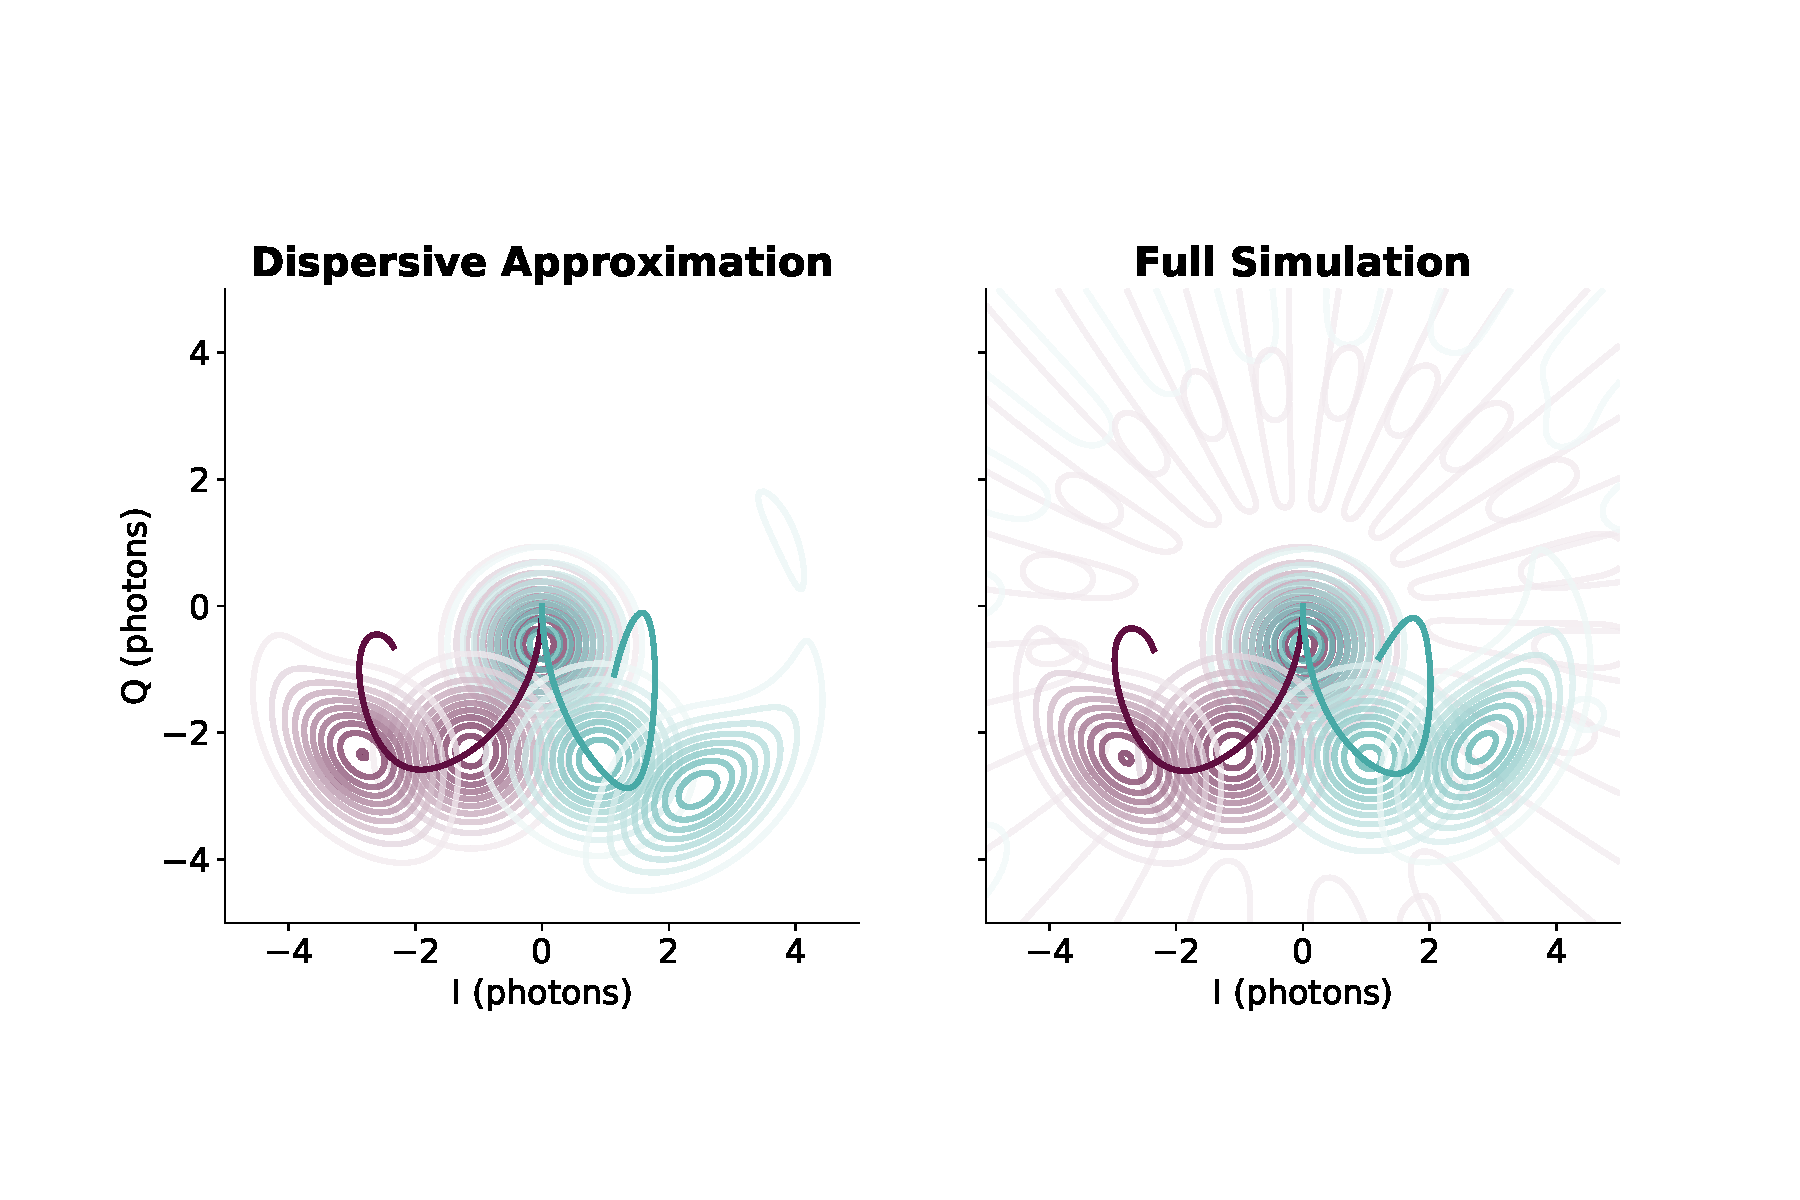
\includegraphics[width = \textwidth]{Simulations/readout_simulations/figures/dispersive_approx.pdf}
    \caption{Simulated readout drive using the dispersive approximation and full time-dependent Hamiltonian. The expectectation value for the I and Q quadratures are shown along with the Q function at three different times.}
    \label{fig:dispersive_slash_full_readout}
\end{figure}

% In the dispersive limit, we consider that $g/(\omega_r - \omega_q) \ll 1$, which has be sufficient for us since we consider low-photon-number readout. If we were to increase this to the high power regime, one starts to see a lot of interesting physics. The point of increasing $n > n_{\text{crit}}$, the approximation is no longer good. Doing the experiment in the laboratory we see that the resonator at some point get completely decoupled from the qubit.

% \begin{marginfigure}
%     \centering
%     \missingfigure{Punchout visualization}
%     \caption{Caption}
%     \label{fig:experiment_punchout}
% \end{marginfigure}

% In this regime the dispersive approximation is definetly wrong and we would have to resort back to the full time-dependent Hamiltonian. However, since the ciritcal photon number is $\approx 400$, we are nowhere near able to run these simulation anyways. 

\FloatBarrier

\subsection{Q Function and Trajectories}
In section \ref{sec:IQ_phase_space}, we introduce the Q-Function to determine the phase space probability of finding the resonator with a specific $I, Q$ value set. With the speed-up and accuracy\footnote{Going from order $1.5 \rightarrow 12$ reduces errors significantly} the Lindblad equation has over the Stochastic Master Equation, one might ask, why we went through the trouble of introducing and coding it. The short answer is that it was a lot of fun. The longer answer requires us to compare the Q function to the measurement trajectories of the Stochastic Master Equation.

As a start, we might have to revisit the interpretation of the density matrix. In the example, we had in section \ref{sec:density_with_env} the mixed state came from someone (or something) measuring our state without our knowledge. This left us with a state that if we repeat the experiment would yield $\ket{0}$ half of the time and $\ket{1}$ in the other half. In the Lindbladian formulation the density matrix can be formulated as an ensemble average, that if we do it multiple times, we would arrive at this outcome. For the SME, we measure it in the meantime. The information here, would no longer be an ensemble average in the same way, but slowly collapse to which of trajectories in the ensemble, we are unraveling. Thus, it can be understood as: if we were to repeat the experiment, with the knowledge that we acquired until now, what is the probability that we have either $\ket{0}$ or $\ket{1}$. \todo{This needs a revisit and probably a source for both the interpretations.}
\begin{figure*}[t]
    \centering
    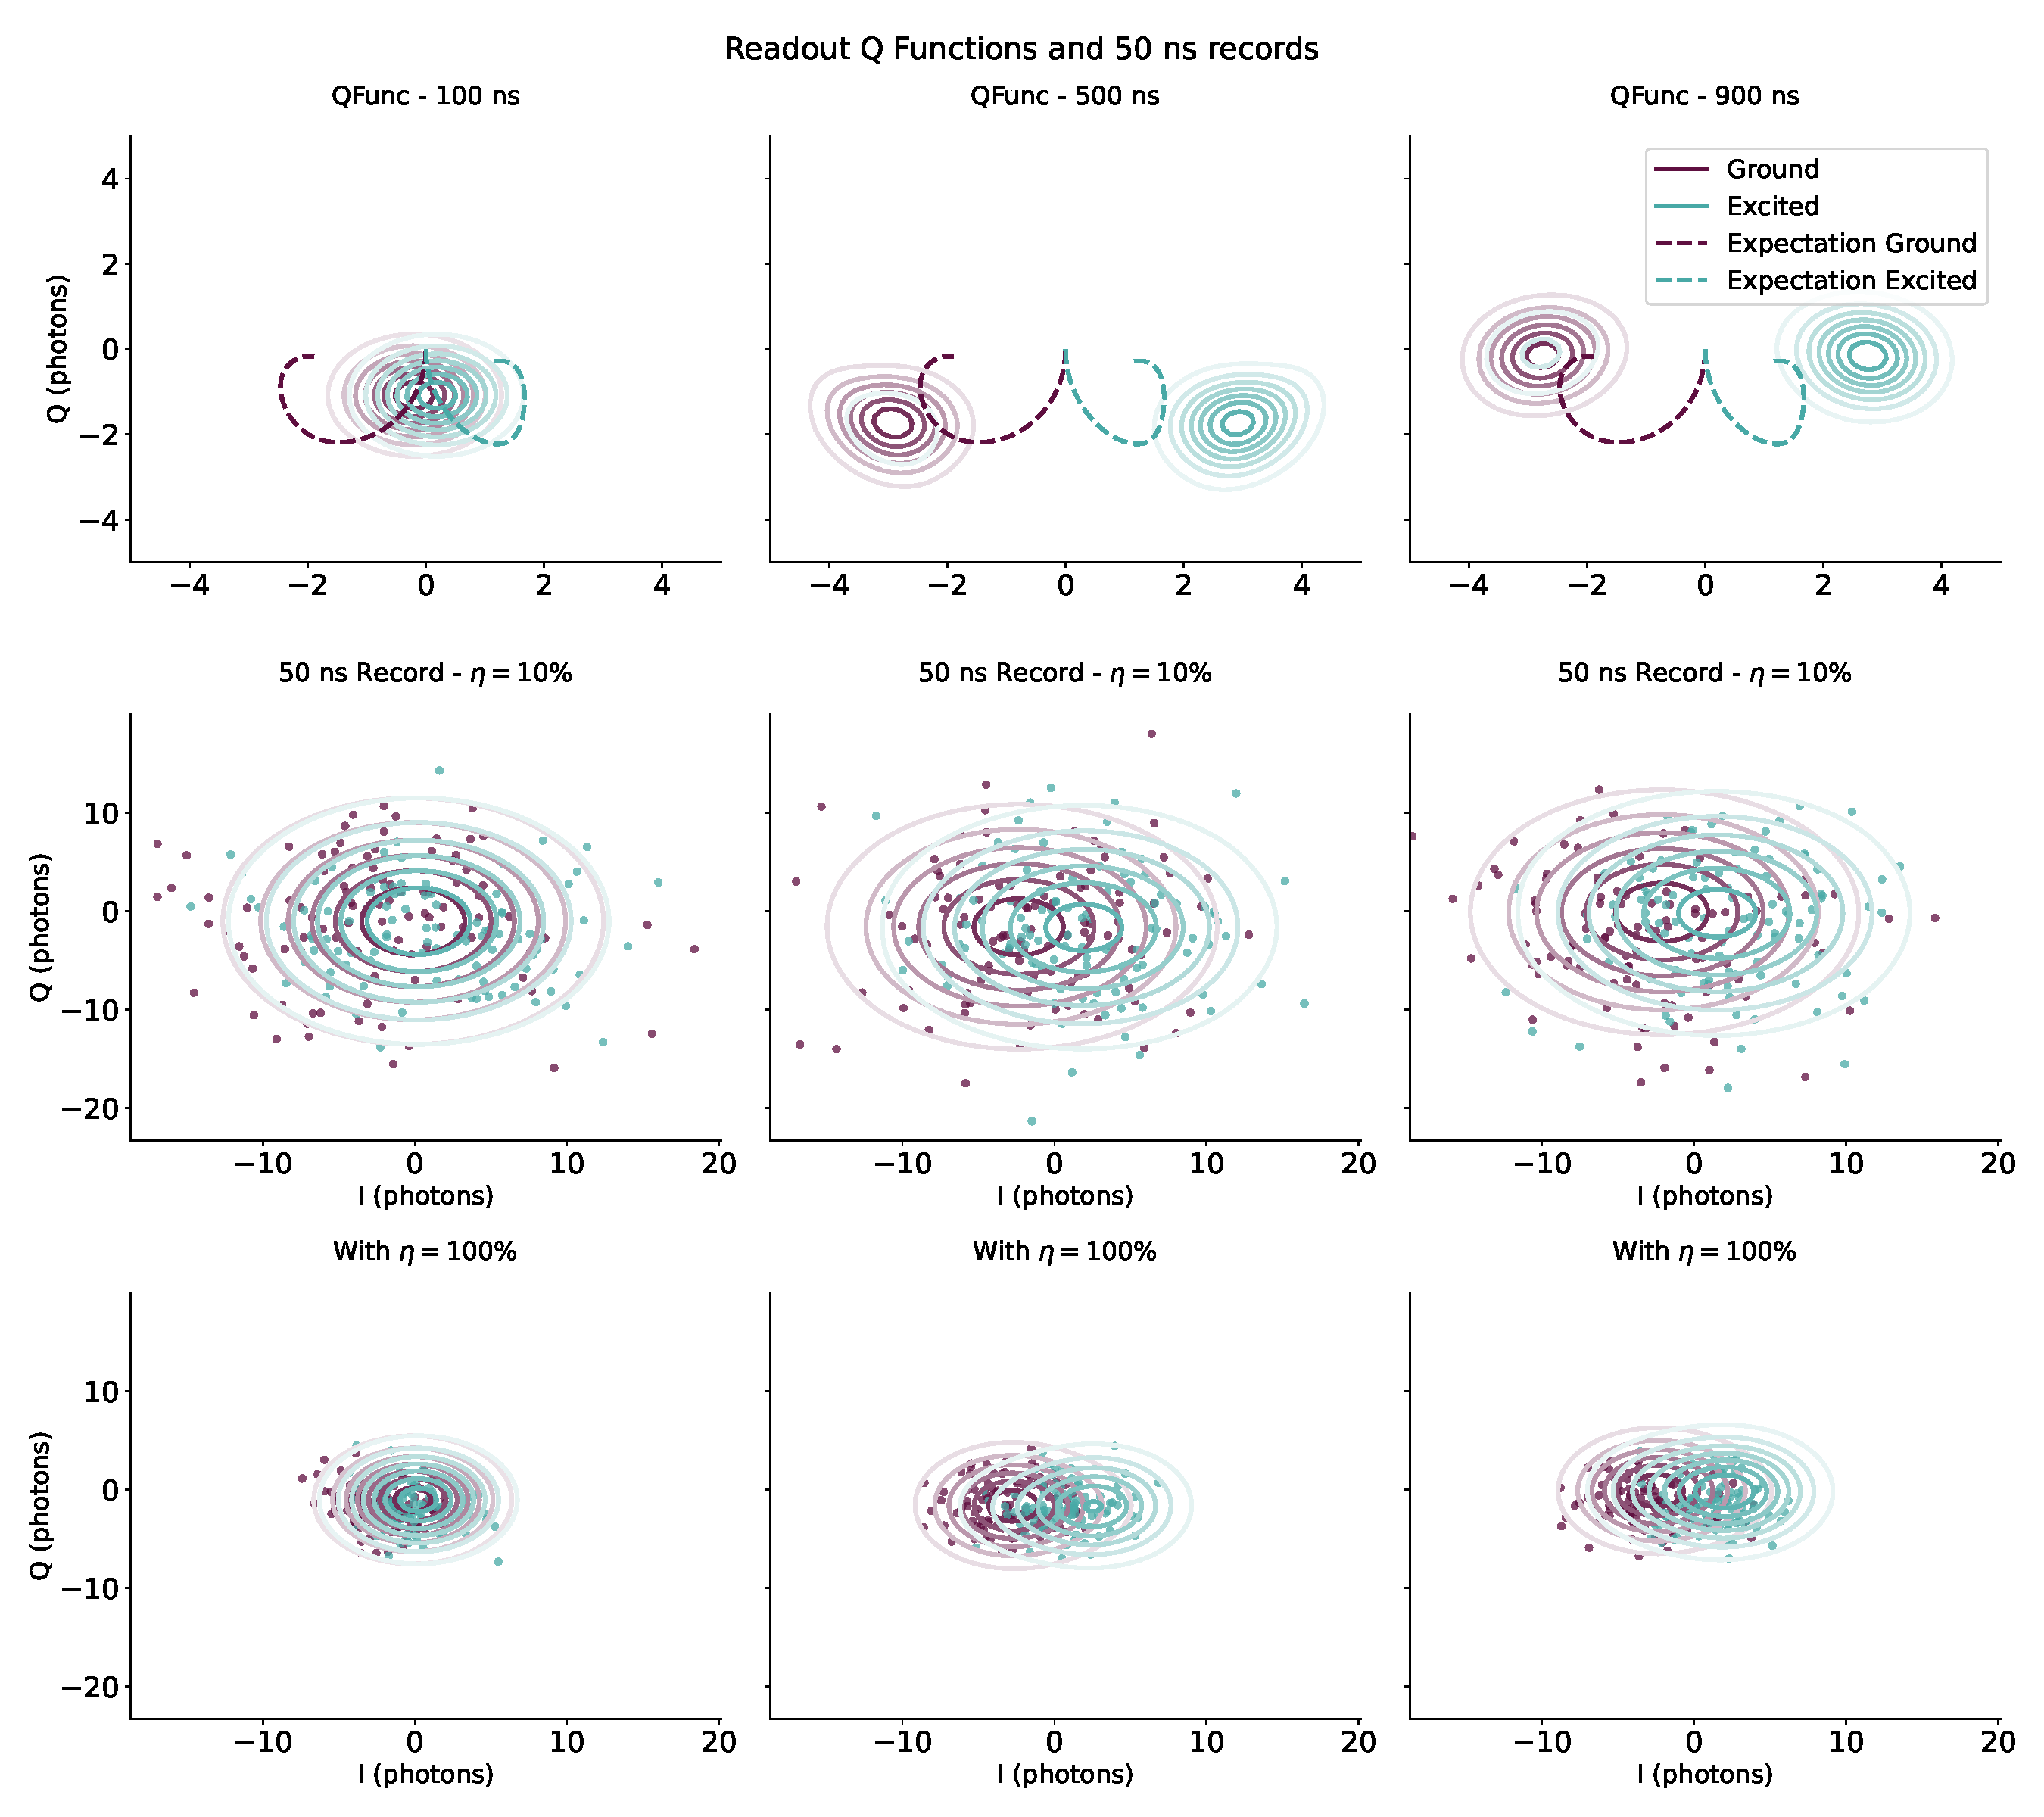
\includegraphics[]{Simulations/readout_simulations/figures/qfunc_trajectories.pdf}
    \caption{Comparison of the Q Function and the scatter plot for a 10 ns readout record. In the top plot the Q Function distribution is shown at $t = 0, 200$ and $400 \text{ ns}$. In the two lower rows the the measurement record for 250 $\ket{0}$ and $\ket{1}$ trajectories are shown. Furthermore, the Q-Function is convolved by a 2d Gaussian with covariance matrix $2 \Delta t / \eta \identity$ to match the error of the records.}
    \label{fig:trajectories_and_qfunc}
\end{figure*}

If we were to not look at the measurement record provided from the measurement\footnote{equal to a measurement with efficiency $\eta = 0$} then the SME reduces to the Lindblad equation, since it described the state, if we obtain no knowledge during the dynamics. It also goes the other way, if we averaged over all possible SME trajectories, we would also be back at the Lindblad equation, and the average measurement record would follow the expectation value of the Lindblad evolved state. If we were to assume that the expectation value of $I$ and $Q$ does not change during a small interval. We could use the Q function distribution and convelute it with the expected Gaussian width of our measurement record. This leads to the distribution of measurements records in that time interval. This is illustrated in \ref{fig:trajectories_and_qfunc}.

This correspondance means that we can use the Lindblad if the interest is in the distribution of records. But we would not be able to create a trajectory by just sampling from the distribution at different time since it do not include the correlation between points as the SME does.
\todo{This section needs a treatment. I think content is good now, but need sources and sharper formulations.}
% \begin{itemize}
%     \item A paragraph: Philosophical differences between measuring and not measuring. Lindblad is the average of many stochastic master equation. This is represented in the mixed state of the density matrix.
%     \item We can covelute the Q function with a Gaussian, which we can find by comparing with the stochastic master equation. This can give the distribution of points at any time.
%     \item The stochastic master equation is necessary for the inter-trajectory correlation. We could sample points from the Q-function, but it would as an example give us 90\% from the $0$ state and $10\%$ for the excited state. However, in reality one trajectory will have 100\% of its measurements from one distribution from just one of them.
% \end{itemize}

% \vspace{1 cm}
% Old $\downarrow$ \\






% When we consider the Lindblad equation, the result is a deterministic list of density matrices at each point in time. This is also a possiblity, when we integrate the Stochastic Master Equation, but in addition, we have the simulated trajectories which resemble the contious weak readout done in the laboratory. In order to compare these two methods, we will make use of the Q-function represented in \ref{sec:QFunc} which illustrates a 2-dimensional probability density of the quadratures in the resonator. 

% If we simulate the readout process of the qubit-resonator system under the dispersive approximation, we can compare the measurement records from the Stochastic Master Equation with the evolution of the Q-function from the Lindblad Equation. This is summarized in figure \ref{fig:trajectories_and_qfunc}


% The measurement record is given by a term proportional to the expectation value of the measured quantity and a noise term, which in the derivation from chapter \ref{sec:} was a Gaussian. For a perfect coherent state, this is closely to the distribution of its Q function. Especially in the hetereodyne measurements. For a state, we can get a somewhat approximation. We need to scale the standard deviation with eta. Furthermore, we get a reductioon depending on the time of the measurement. This gives the good idea of measuring.... \todo{This is really just me writing sentences which could be included}






\section{Timesteps and the Size of the Hilbert Space}\label{sec:hilbert_space}
To complete our simulation tool, we still have to decide on the proper size of the Hilbert Space and the size of the time steps. 

The time-step size is probably the easier. One trick in Qutip is that the Adams algorithm actually calculates a 13th order integration step. If the Taylor series converges, then the difference between the 13. and 12. order term will be larger than the leftover error and we can set a threshold on the accuracy we accept \cite{KALKULUS}. Qutip allows for up to 2500 substeps per timestep and if the error is still to large it terminates and raises an error \cite{johansson_qutip_2012}. This means, we should just set the resolution to the lowest without raising an error. To be safe, we set it a bit higher and simulate the readout of $600 \text{ ns}$ in $10 \text{ ns}$. %\todo{The Adams algorithm further allows up to a certain amount of subcalls to algorithm which is adjusted based on the error}

The Taylor Milstein 1.5 scheme also checks error bounds. With the stochastic term it is however not as reliable and with a low time resolution the measurement records included NaN values. A resolution which seems to work is running $2 \text{ ns}$ when the efficiency is low, and increasing the resolutino to $1 \text{ ns}$ when testing the efficiencies $\eta > \frac13$. 

% \begin{figure*}
%     \centering
%     \missingfigure{Something showing hilbert space problems}
%     \caption{Caption}
%     \label{fig:enter-label}
% \end{figure*}
The size of the Hilbert Space affects the complexity of the simulation significantly, since the entries of the density matrix scales as $n^2$ with $n$ the dimension of the Hilbert Space. However, picking the size is like most of these considerations a trade off between accuracy and speed of simulations. 

For the Qubit we need to have at a two dimensional system but we have include a third to be able to calculate the dispersive shift when we are doing the full model. This would further allow for transitions leakage to and from the excited state. This is however not fully implemented in the models yet since the occupancy would be $<1\%$ with temperatures around $140$ mK making it less of a priority. \todo{Do the calculation to confirm!} 

For the resonator, we have to make sure, we do not miss any of the dynamics. Thus the size of the Hilbert space should be significantly larger than the maximum number of photon, we will have at any point during the simulation. The coherent states are decomposed into fock space states near the mean photon number. With the values of $\kappa$ and $\chi$ in our system, the resonator does not directly enter the steady state, but overshoots it by a bit\footnote[][1 cm]{We saw this when calculating the trajectories in section \ref{sec:resonator_decays}}. When we further add the stochastic nature in the SME, we had to increase it even more to make sure, we do not get near the border. With resonator hilbert space of dimension 50 seemed to include all the desired effects without being to large. Again a few trajectories with high $\eta$ has some numerical problems which results in incorrect movements in the IQ plane. 

\section{Readout in Simulation}\label{sec:readout_in_simulation}
With calibrated device parameters, implemented simulations, trust in the dispersive model and the numerical settings, we are ready to do the readout simulations. By using the SME with the dispersive model and the parameters calibrated and summarized in section \ref{sec:overview_section}, we recreate the readout experiment from chapter \ref{chap:readout}. We create 500 trajectories for the equilibrium state calculated from the temperature and 500 times with an x-gate applied to the equilibrium state.

The IQ trajectories was combined with optimal weights and the maximum separating line was found. The process can be seen in figure \ref{fig:simulation_readout} where we remember that the phase of the IQ plot is our choice, so we are free to rotate it when comparing with figure \ref{fig:readout_process}. The state initialization and measurement error of our readout process in the simulated system is:
\begin{equation}
    F_{\text{SPAM}} = 0.654 \pm 0.024
\end{equation}
Which is close to the actual experiment. Comparing the two, we find a $z$-score\sidenote{$|F_e - F_s| / \sqrt{\sigma_s^2 + \sigma_e}^2$ where subscript e is the fidelity and error of the experiment and s is for simulation} of 1.33. A fidelity from the same distribution as the experiment would have probability of  $p = 18.4 \%$ of being further from the actual value. This is a good indication that we are on the right track. Even though we still have multiple additions left. This includes the ramp-up and down of the experimental readout pulse, a realistic X-gate and proper inclusion of the dynamics associated with the second excited state. 
\begin{figure*}[t]
    \centering
    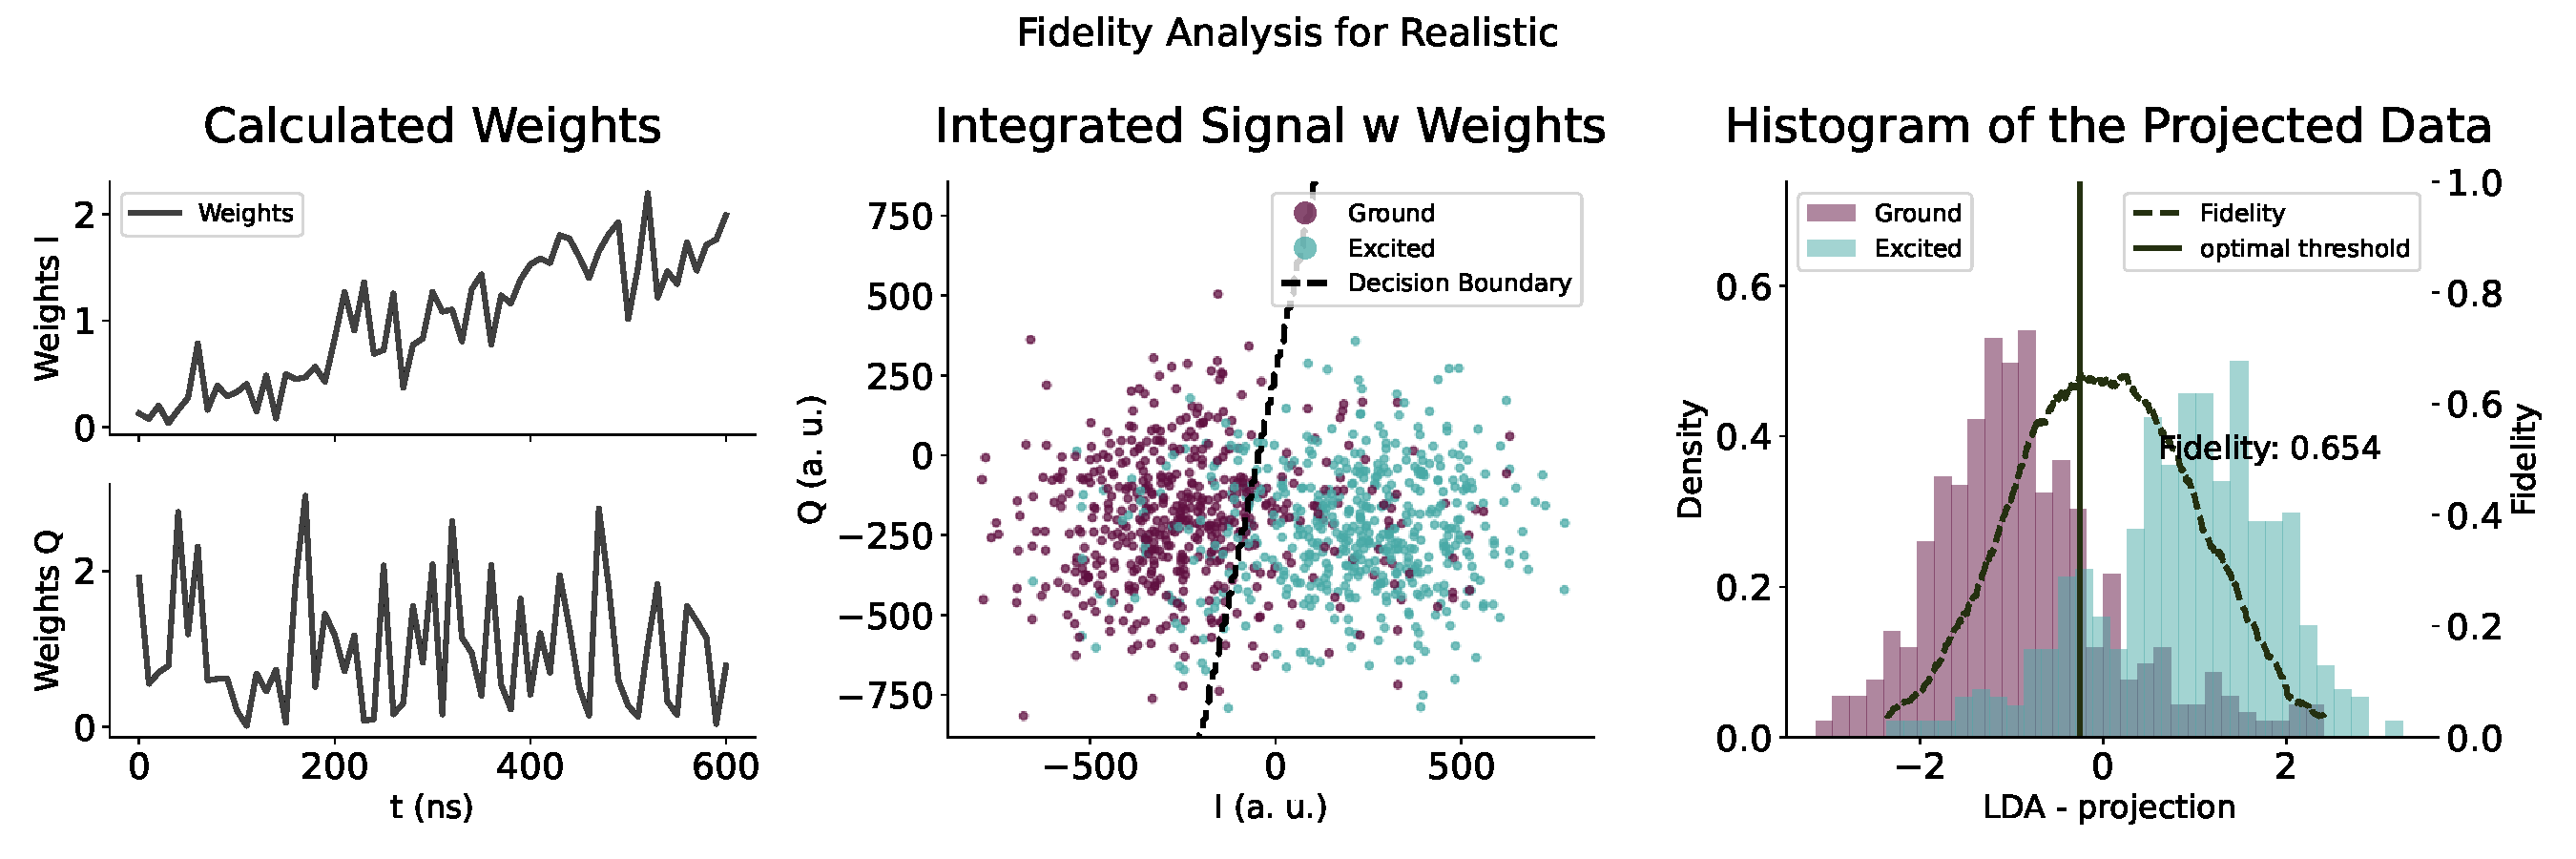
\includegraphics[]{Simulations/budgets/figures/realistic_sme.pdf}
    \caption{The weights, IQ plots and a histrogram of the simulated dataset. The histogram is combined with the fidelity of setting a threshhold at the particular value. The maximum is chosen.}
    \label{fig:simulation_readout}
\end{figure*}


\begin{table}[h]
    \centering
    \begin{tabular}{c|cc}
                & KS-statistic & pval  \\ \hline
    Full        & 0.036 & 0.367         \\
    Ground      & 0.075 & 0.046         \\
    Excited     & 0.072 & 0.062
    \end{tabular}
    \caption{Caption}
    \label{tab:my_label}
\end{table}

\begin{figure}
    \centering
    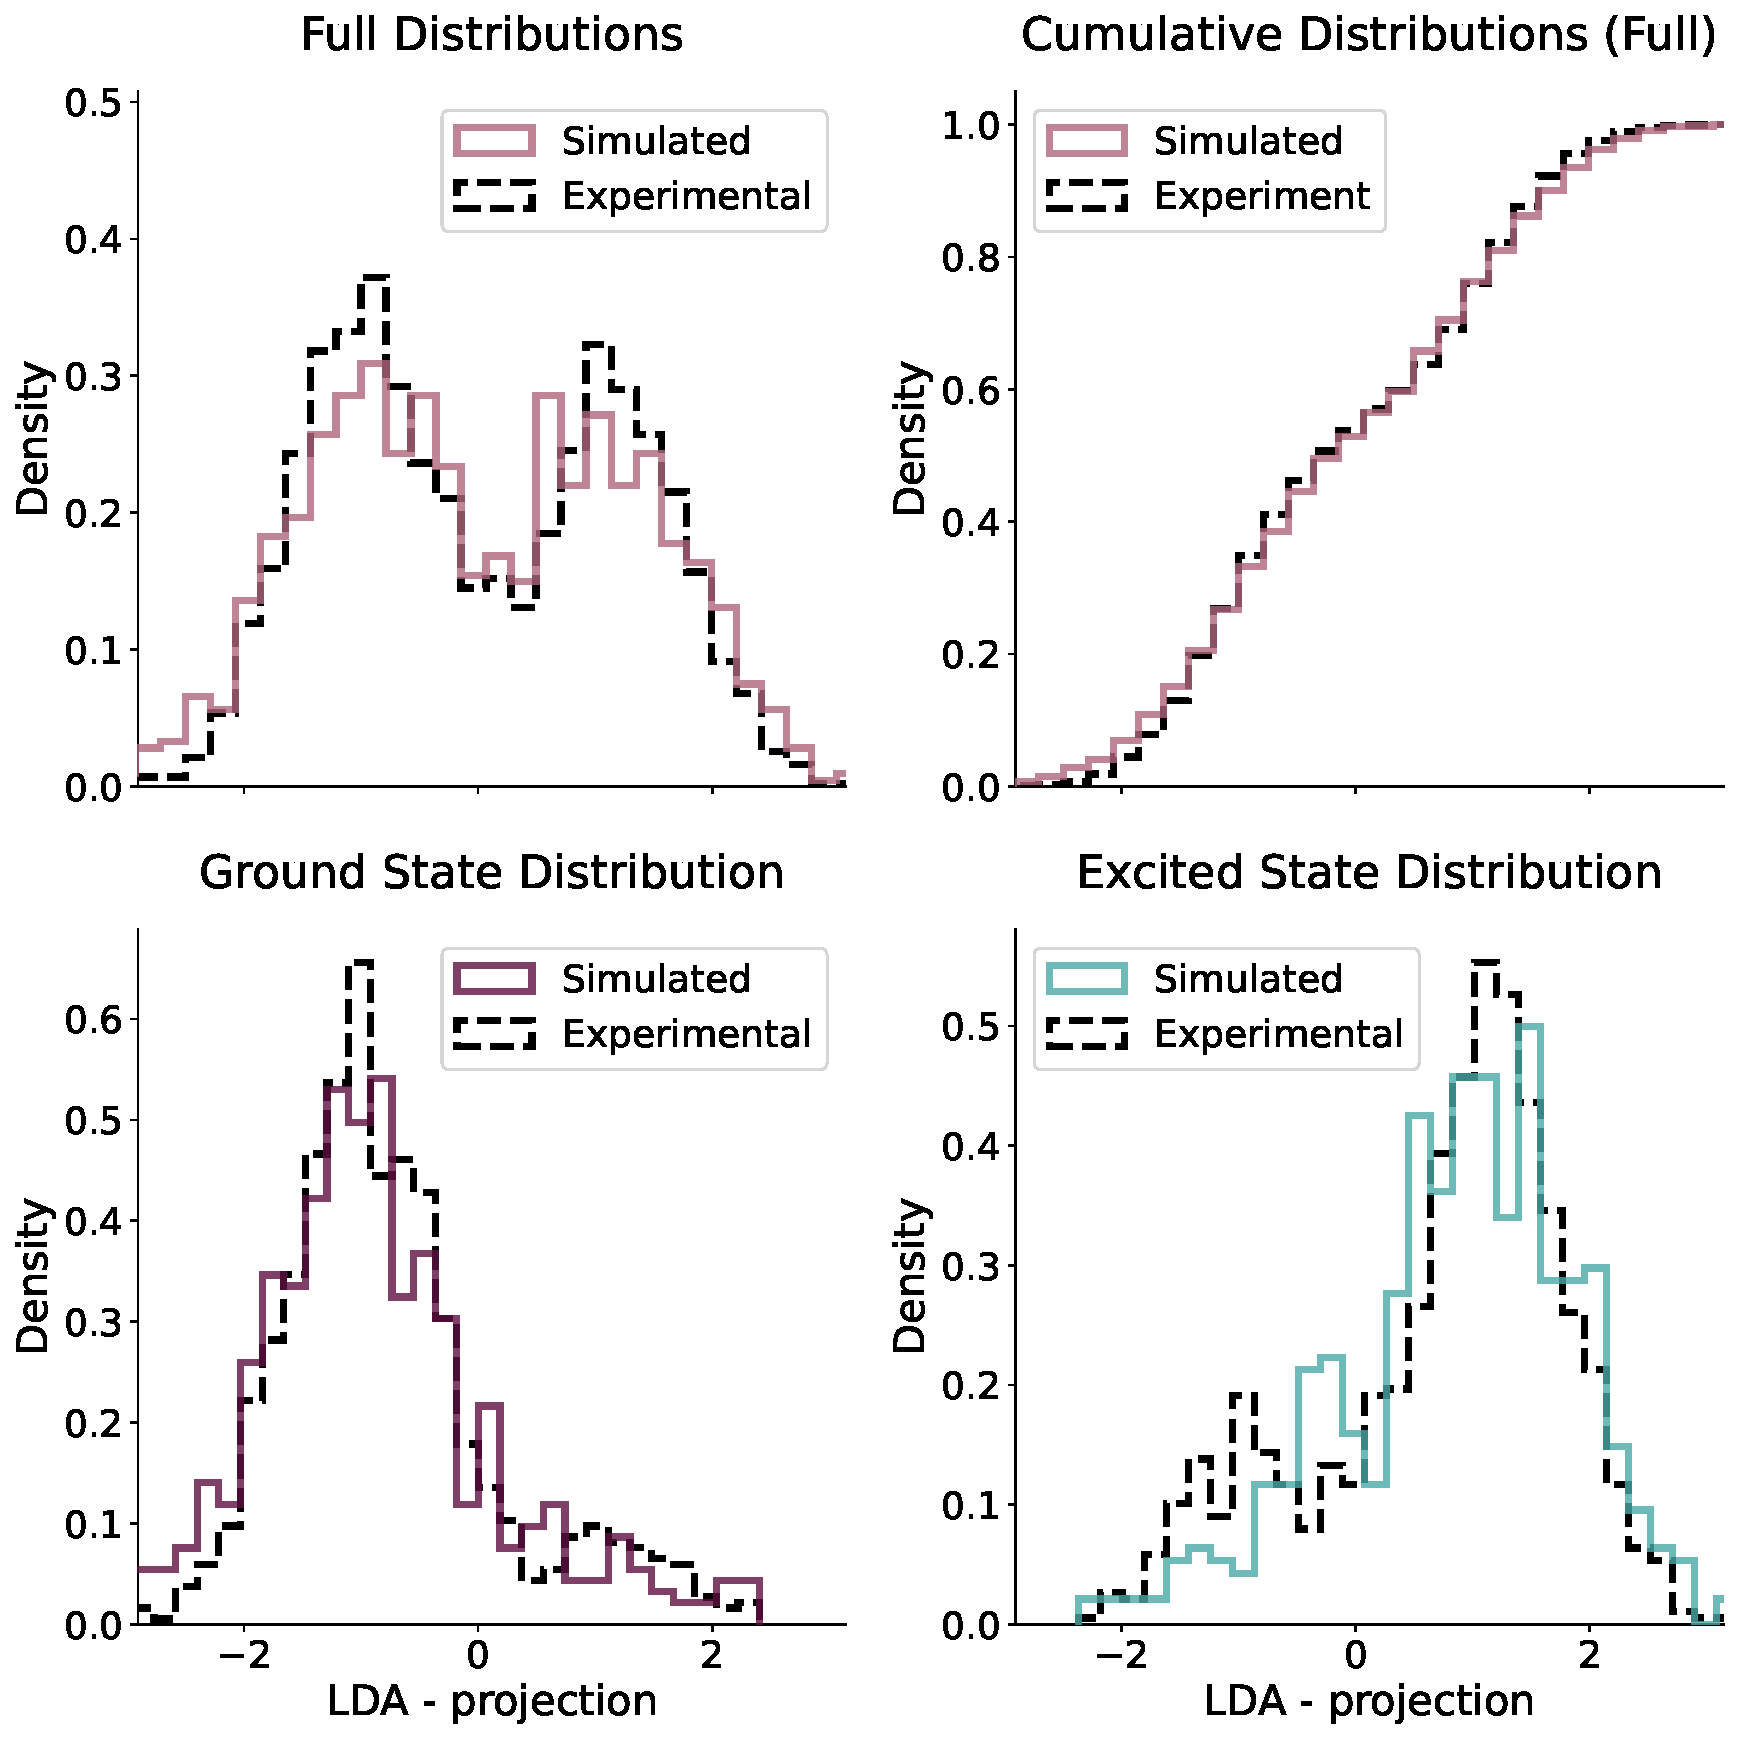
\includegraphics{Readout/Figs/Weighted_comparison_with_simmulation.pdf}
    \caption{Caption}
    \label{fig:enter-label}
\end{figure}


\todo{calculate the two tailed sf again with the correct error on the fidelity}